\begin{figure*}[!h]
        \centering
        \begin{subfigure}[b]{0.32\textwidth}
            \centering
            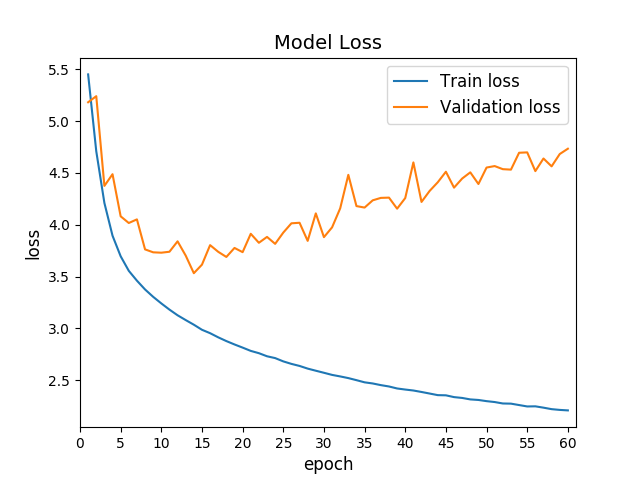
\includegraphics[width=\textwidth]{../images/final_loss.png}
            \caption[]%
            {{\small }}
        \end{subfigure}
        \hfill
        \begin{subfigure}[b]{0.32\textwidth}
            \centering
            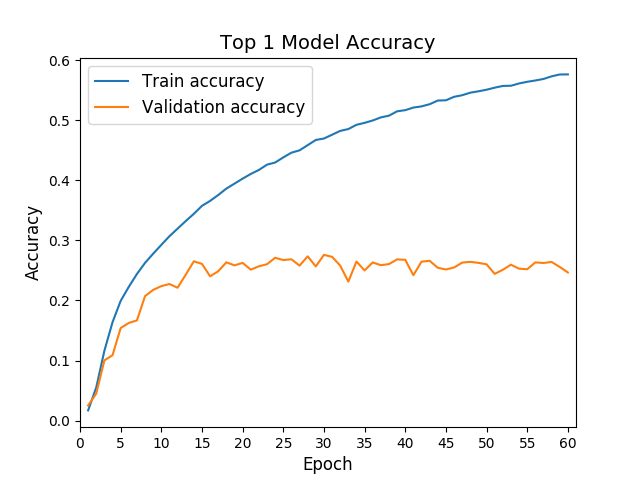
\includegraphics[width=\textwidth]{../images/final_top1.png}
            \caption[]%
            {{\small }}
        \end{subfigure}
        \hfill
        \begin{subfigure}[b]{0.32\textwidth}
            \centering
            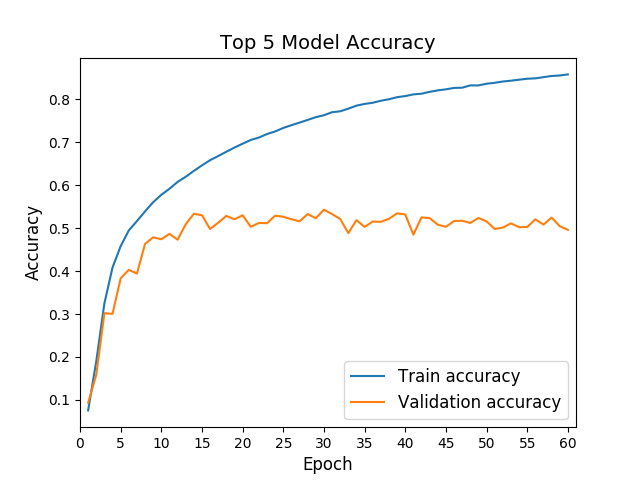
\includegraphics[width=\textwidth]{../images/final_top5.png}
            \caption[]%
            {{\small }}
        \end{subfigure}
        \caption[]
        {\small Training and validation loss of 60 first epochs from model E, specified in \ref{table:final2configs}. (a) Training and validation loss. (b) Training and validation top-1 accuracy. (c) Training and validation top-5 accuracy.}
        \label{fig:final_plots_e}
    \end{figure*}
\FloatBarrier
